\chapter{Results}
\begin{enumerate}
\item Metrics: PSNR, (Relative Error), (FSIM)
\item Full Res vs Pre-compressed: With full res, I need a lot of samples to get perfect reconstruction. With pre-comp, I'm not sure.
\item Curve: Performance vs Compression
\item Masks vs Gaussian vs Rademacher
\item Haar vs DCT (vs Daub)
\item What't the best performance I can achieve? How does it compare to the lit?
\item .
\item MSCE was done to solve the signal interpolation. In particular, to fix the problem with small support of wavelets while still using their power.
\item Problem: Slow. Solution: Parallelization.
\item Problem: Limited to signal interpolation. Solution: Use CS sensing matrices (but Cascade don't work yet).
\item Do we even need the cascade? What if we jump straight to the third scale.
\item Can we improve the performance of the interpolator? 
\end{enumerate}

We have obtained some results with our current implementation.
The implementation uses the Haar wavelet transform at the first scale.

Our example video has a resolution of 128 by 128 pixels and consists of a total of 64 frames.
Thus, $r = 128$, $c = 128$ and $s = 64$.
Note that even for such a relatively small sample, the size of the basis matrix $\Psi$ is $(128*128*64)\times(128*128*64) = 1048576\times 1048576$.
Even in single precision, storing this matrix would require around 4 terrabytes.

For this reason, we have split the original input signal into $8\times 8\times 8$ blocks and perform the algorithm on the individual blocks.
\begin{figure}
\label{fig:foreman}
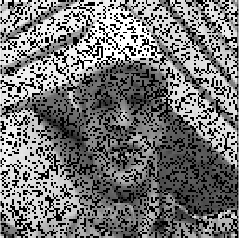
\includegraphics{Images/corr.png}
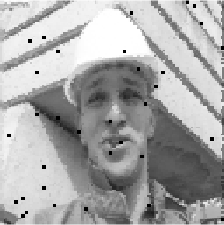
\includegraphics{Images/rec.png}
\caption{Sample frame from corrupted video (left) and the reconstructed video (right)}
\end{figure}

\begin{figure}
\label{fig:soccer}
\center
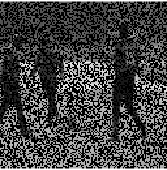
\includegraphics{Images/corr2.png}
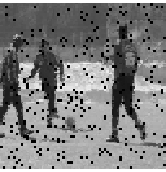
\includegraphics{Images/rec2.png}
\caption{Sample frame from corrupted video (left) and the reconstructed video (right)}
\end{figure}

In Figures 3.1 and 3.2, we have included a sample frame from the corrupted test video and the same frame after reconstruction.

In Figure 3.1, we corrupted the video by deleting 30\% of the pixel values in the first frame and deleting the same pixel values in each subsequent frame (so the same pixels are missing in each frame).
Figure 3.2 uses the same corruption scheme but we deleted 50\% rather than 30\% of pixel values.

These initial results are promising, though clearly there are still improvements to be made.

